\documentclass[10pt]{article}
\usepackage[ngerman]{babel}
\usepackage[utf8]{inputenc}
\usepackage[T1]{fontenc}
\usepackage{graphicx}
\usepackage[export]{adjustbox}
\graphicspath{ {./images/} }
\usepackage{hyperref}
\hypersetup{colorlinks=true, linkcolor=blue, filecolor=magenta, urlcolor=cyan,}
\urlstyle{same}

\title{Bachelor of Science (BSc) in Informatik Modul Software-Entwicklung 1 (SWEN1) }

\author{}
\date{}


%New command to display footnote whose markers will always be hidden
\let\svthefootnote\thefootnote
\newcommand\blfootnotetext[1]{%
  \let\thefootnote\relax\footnote{#1}%
  \addtocounter{footnote}{-1}%
  \let\thefootnote\svthefootnote%
}

%Overriding the \footnotetext command to hide the marker if its value is `0`
\let\svfootnotetext\footnotetext
\renewcommand\footnotetext[2][?]{%
  \if\relax#1\relax%
    \ifnum\value{footnote}=0\blfootnotetext{#2}\else\svfootnotetext{#2}\fi%
  \else%
    \if?#1\ifnum\value{footnote}=0\blfootnotetext{#2}\else\svfootnotetext{#2}\fi%
    \else\svfootnotetext[#1]{#2}\fi%
  \fi
}

\begin{document}
\maketitle
\section*{LE 05 - Softwarearchitektur und Design I}
SWEN1/PM3 Team:\\
R. Ferri (feit), D. Liebhart (lieh), K. Bleisch (bles), G. Wyder (wydg)

\section*{Um was geht es?}
\begin{itemize}
  \item Wie kann ich eine logische Architektur aus den Anforderungen ableiten?
  \item Welche Architekturpatterns gibt es?
  \item Wie kann ich Architekturentscheide herleiten und dokumentieren
  \item Wie modelliere ich meine logische Architektur mit der UML, um sie diskutieren und evaluieren zu können?\\
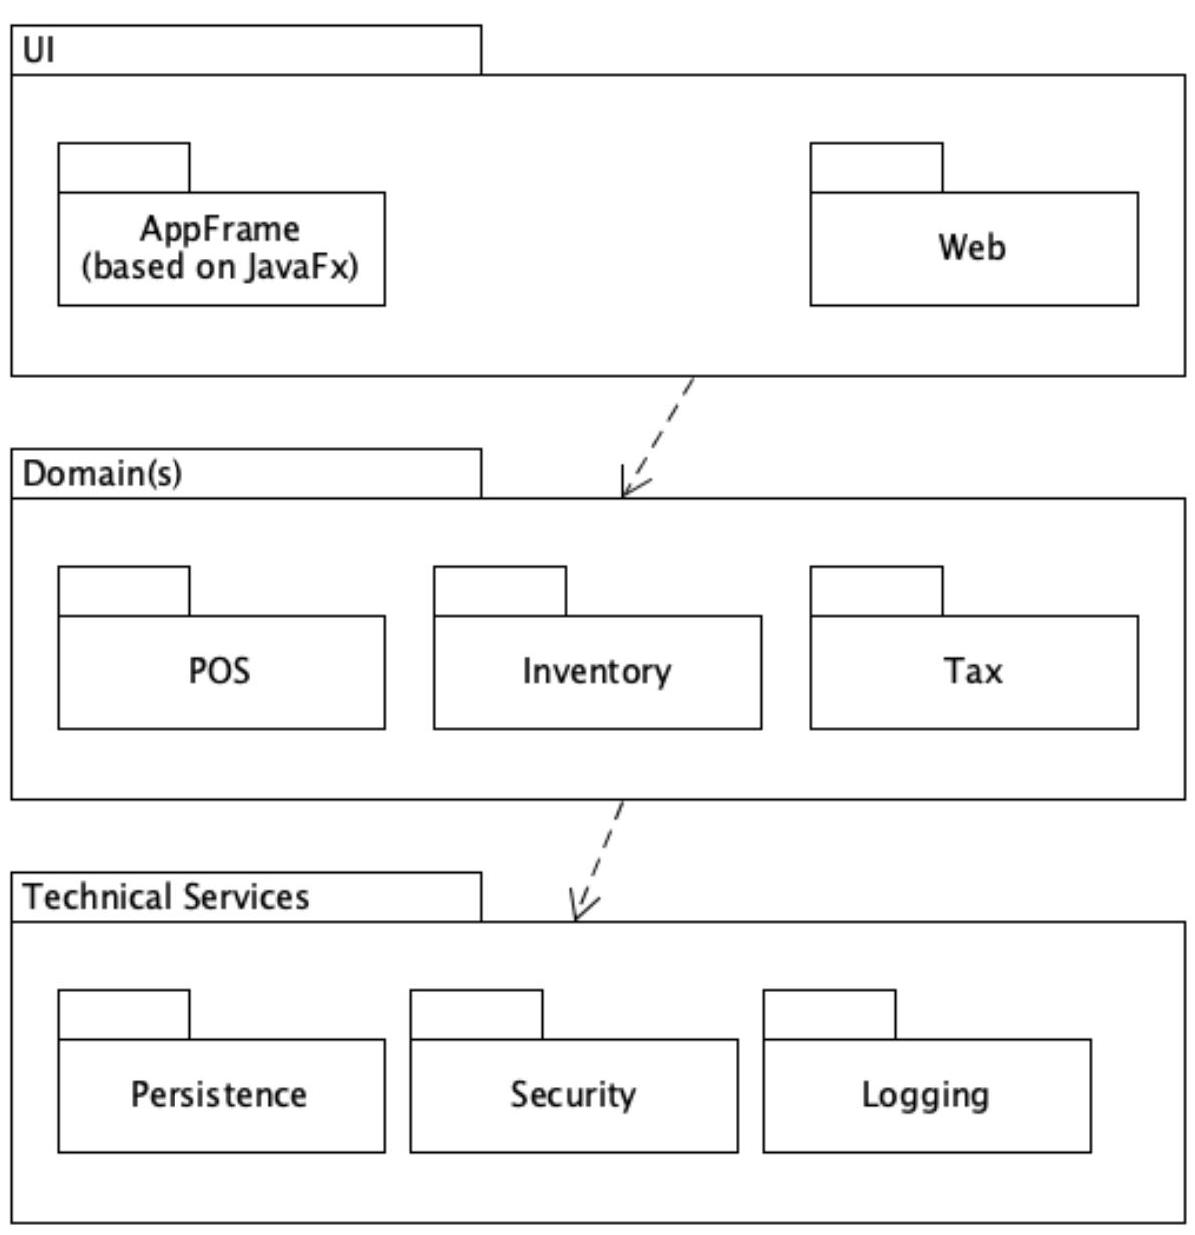
\includegraphics[max width=\textwidth, center]{2025_01_02_bc08e794b8341102ce21g-02}
\end{itemize}

\section*{Lernziele LE 05 - Softwarearchitektur und Design I}
\begin{itemize}
  \item Sie sind in der Lage,
  \item die Bedeutung der logischen Architektur zu erläutern,
  \item die Einflussfaktoren aus den nicht-funktionalen Anforderungen für die logische Architektur abzuleiten,
  \item den Aufbau von UML-Paketdiagrammen zu erklären,
  \item das Schichten-Entwurfsmuster zu beschreiben,
  \item die wichtigsten Architekturpatterns zu nennen.
\end{itemize}

\section*{1. Was ist eine Softwarearchitektur}
\begin{enumerate}
  \setcounter{enumi}{1}
  \item Architektur aus den Anforderungen ableiten
  \item Modulkonzept
  \item Architekturen beschreiben
  \item UML-Paketdiagramme
  \item Ausgewählte Architekturpatterns und Beispielarchitekturen
  \item Aufgaben eines Software-Architekten
  \item Wrap-up und Ausblick
\end{enumerate}

\section*{Was ist Softwarearchitektur?}
\begin{itemize}
  \item Gesamtheit der wichtigen Entwurfs-Entscheidungen
  \item Programmiersprachen, Plattformen
  \item Aufteilung des Gesamtsystems in Teilsysteme, Bausteine samt deren Schnittstellen
  \item Verantwortlichkeiten der Teilsysteme und ihre Abhängigkeiten
  \item Einsatz einer Basis-Technologie oder eines Frameworks, z.B. Java EE
  \item Besondere Massnahmen, um Anforderungen erfüllen zu können
  \item Z. B. redundante Datenspeicherung
  \item Grundlagen
  \item Anforderungen (vor allem nicht-funktionale)
  \item Systemkontext mit Schnittstellen
  \item Top Level View (das grosse Ganze)\\
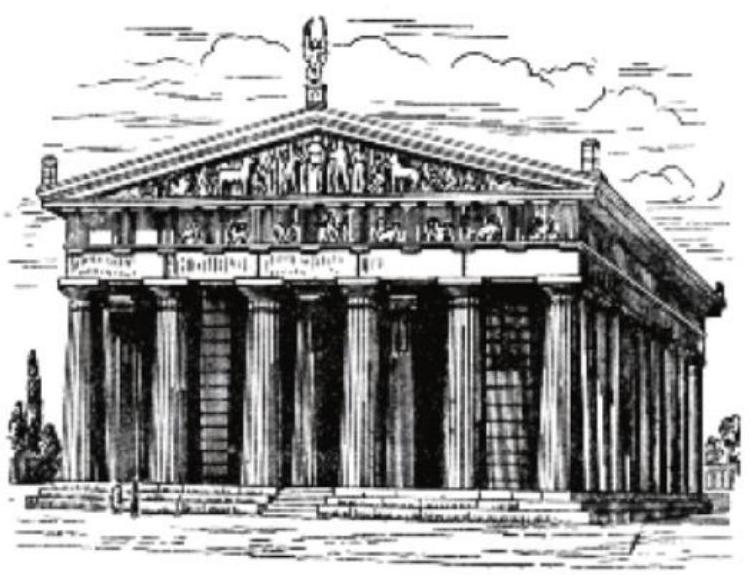
\includegraphics[max width=\textwidth, center]{2025_01_02_bc08e794b8341102ce21g-05}
\end{itemize}

\section*{Übersicht Business Analyse vs. Architektur vs. Entwicklung}
(1) Domänenmodell (Business Modelling) Kontext Diagramm (Business Analyst)\\
Requirements (Business Analyst)

\begin{itemize}
  \item Liste der Stakeholder
  \item Vision
  \item Funktionale Anforderungen: Use Cases oder User Stories
  \item Nichtfunktionale Anforderungen: Supplementary Specification
  \item Randbedingungen
  \item Glossar\\

\includegraphics[max width=\textwidth, center]{2025_01_02_bc08e794b8341102ce21g-06(2)}
\end{itemize}

Business\\
Modeling

Require-\\
ments\\
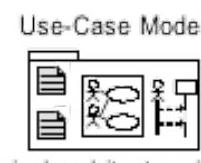
\includegraphics[max width=\textwidth, center]{2025_01_02_bc08e794b8341102ce21g-06(1)}\\
logical architecture is influenced by the constraints and non-functional require ments captured in the Supp. Spec.\\

\includegraphics[max width=\textwidth, center]{2025_01_02_bc08e794b8341102ce21g-06}

\section*{Übersicht Business Analyse vs. Architektur vs. Entwicklung}
(3) Logische Architektur (Software Architekt) Umsetzung (Entwicklung)

\begin{itemize}
  \item Use Case / User Story Realisierung
  \item Anwendung von GRASP
  \item DCD - Design-Klassen-Diagramm
  \item Interaktionsdiagramme
  \item Programmierung
  \item Erstellen der Unit- / Integrations-Tests\\
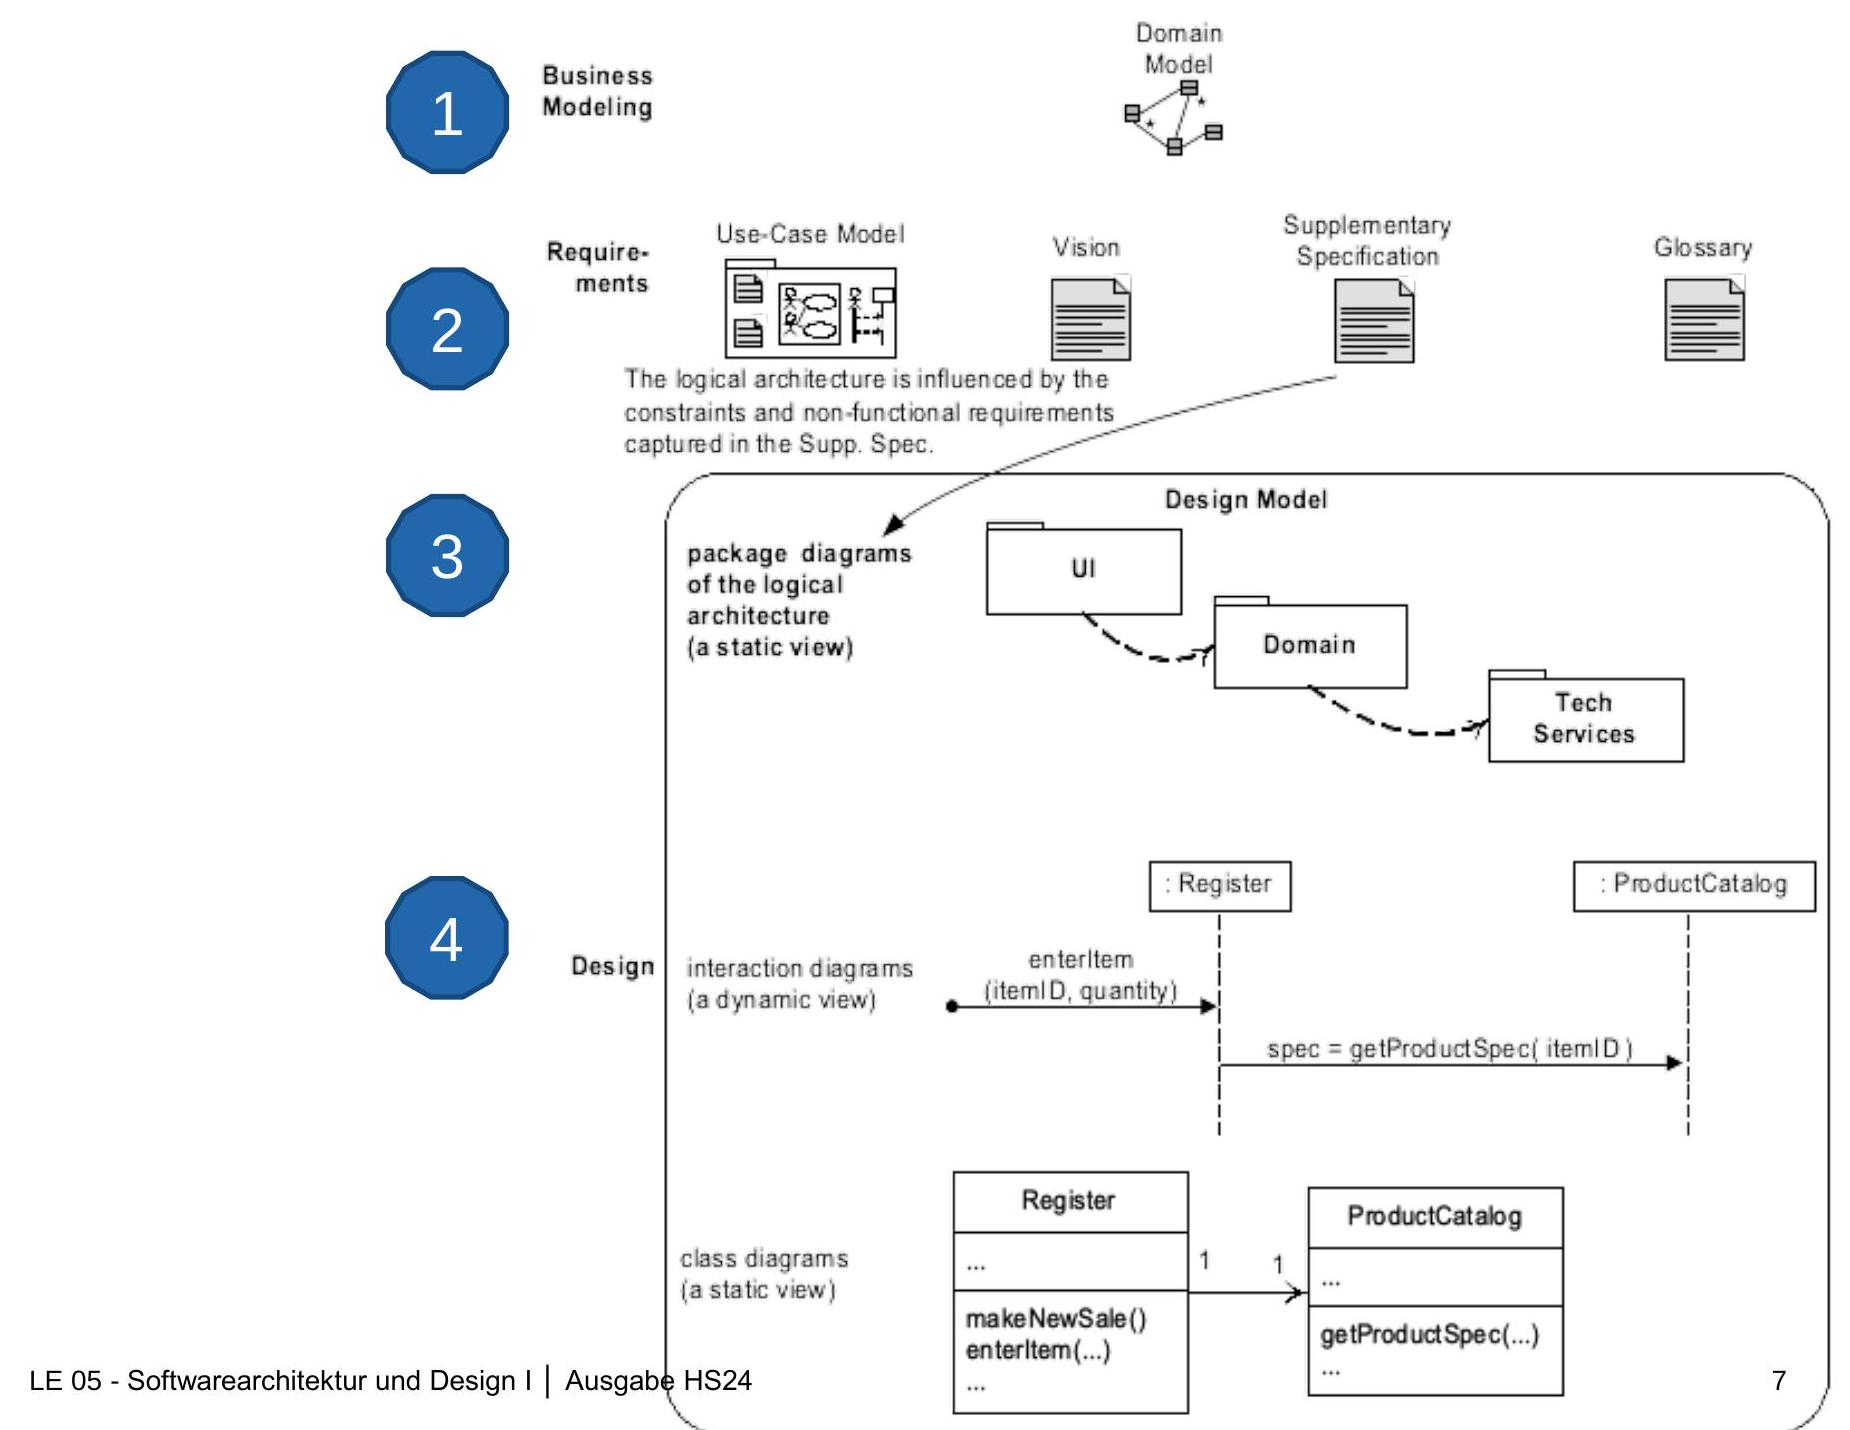
\includegraphics[max width=\textwidth, center]{2025_01_02_bc08e794b8341102ce21g-07}
\end{itemize}

\begin{enumerate}
  \item Was ist eine Softwarearchitektur
  \item Architektur aus den Anforderungen ableiten
  \item Modulkonzept
  \item Architekturen beschreiben
  \item UML-Paketdiagramme
  \item Ausgewählte Architekturpatterns und Beispielarchitekturen
  \item Aufgaben eines Software-Architekten
  \item Wrap-up und Ausblick
\end{enumerate}

\section*{Architektur aus den Anforderungen ableiten}
\begin{itemize}
  \item Die Architektur muss heutige und zukünftige Anforderungen erfüllen können und Weiterentwicklungen der Software und seiner Umgebung ermöglichen
  \item Zentrale Aufgabe der Architekturanalyse
  \item Analyse der funktionalen und insbesondere nichtfunktionalen Anforderungen im Hinblick auf die Konsequenzen für die Architektur
  \item Unter Berücksichtigung der Randbedingungen und ihrer zukünftigen Veränderungen
  \item Dabei müssen Qualität und Stabilität der Anforderungen selbst überprüft werden.
  \item Lücken in den Anforderungen müssen aufgedeckt werden.
  \item Gerade bei den nichtfunktionalen Anforderungen muss hier noch meist nachgebessert werden, da die Anforderungsträger diese häufig als selbstverständlich verstehen.
\end{itemize}

\section*{Nichtfunktionale Anforderungen gemäss ISO 25010}
\begin{center}
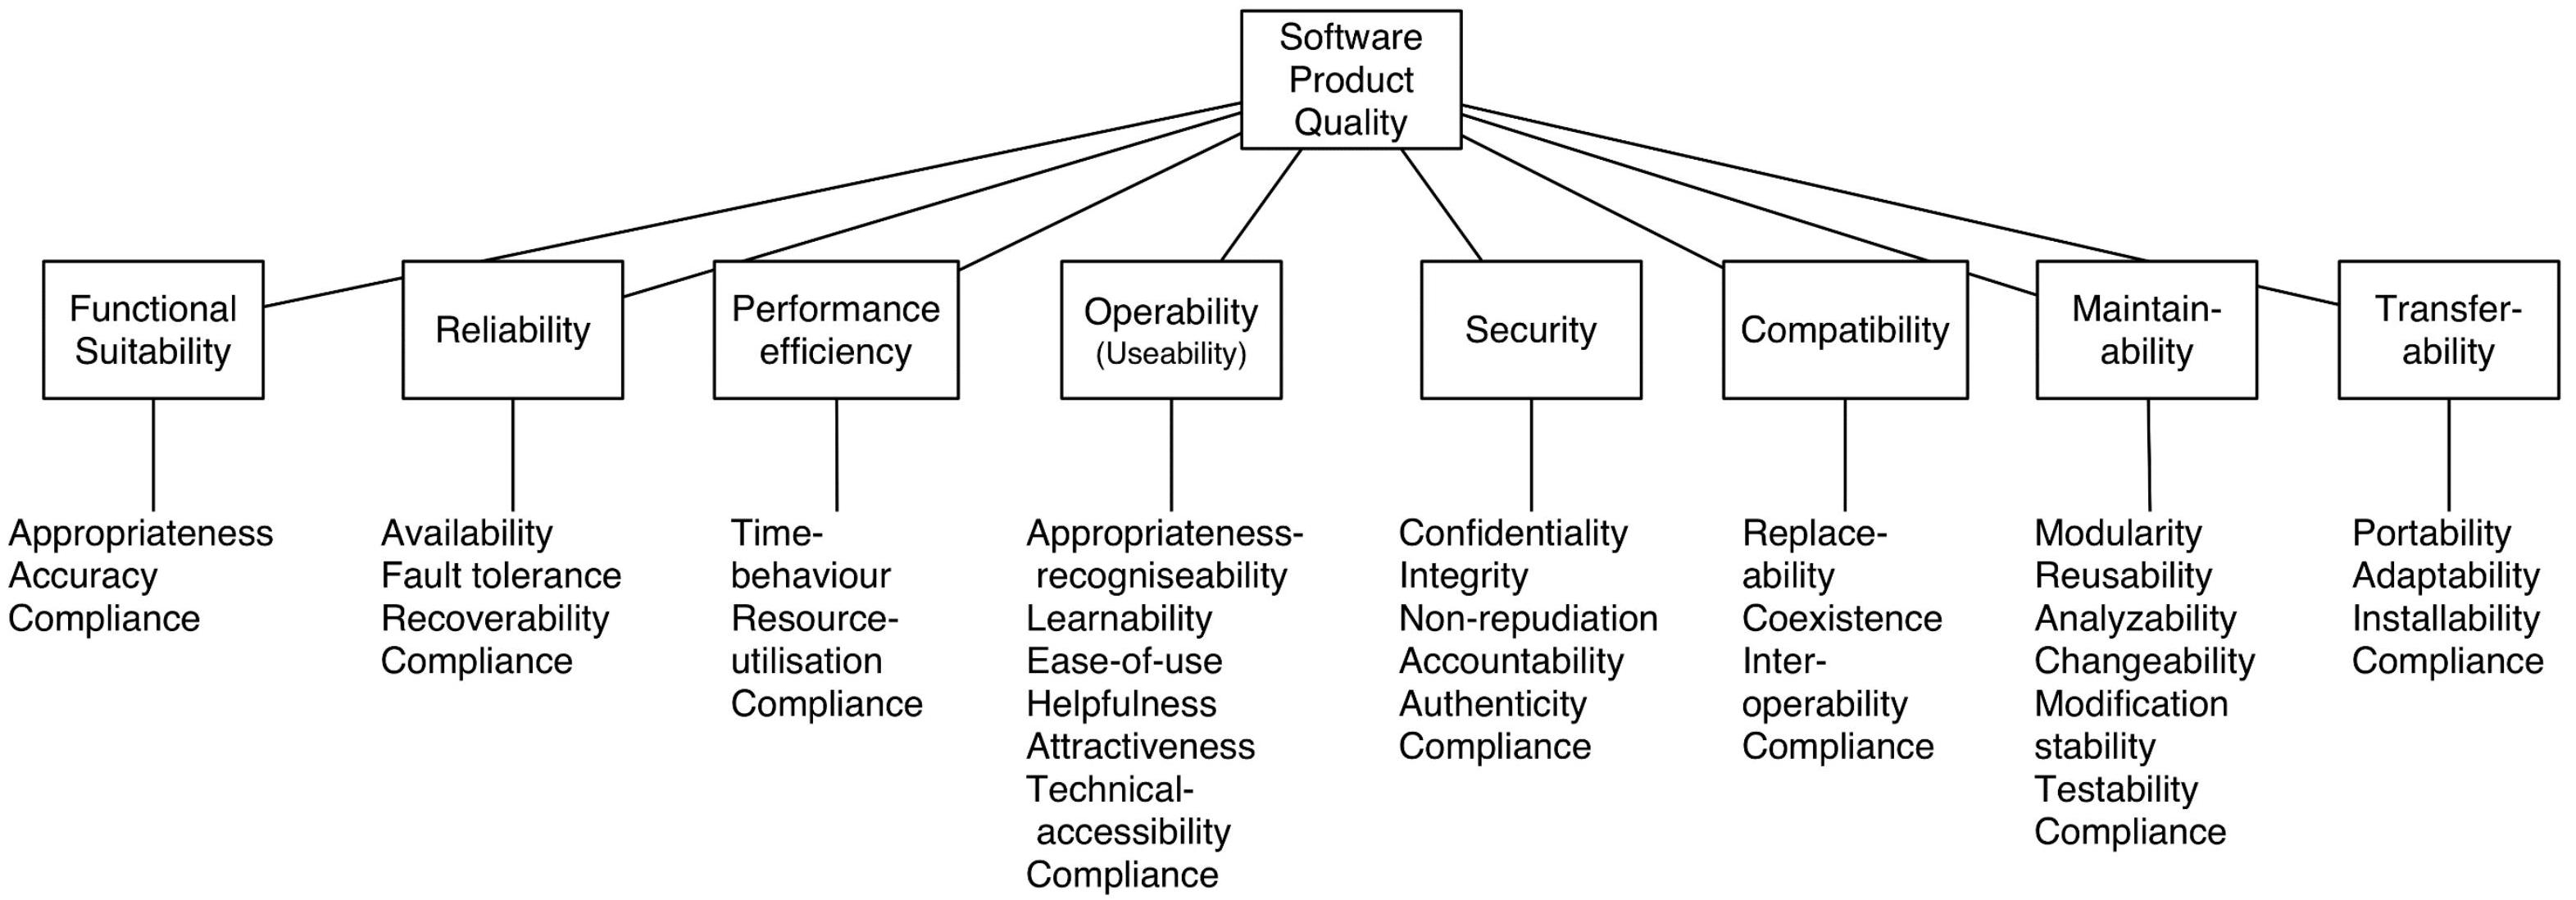
\includegraphics[max width=\textwidth]{2025_01_02_bc08e794b8341102ce21g-10}
\end{center}

\begin{itemize}
  \item Muss Erfüllung der Anforderungen unter den gegebenen Randbedingungen ermöglichen
  \item Heutige und zukünftige Anforderungen
  \item Heutige Randbedingungen und deren zukünftige Veränderung
  \item Grundprinzip
\end{itemize}

Aufteilung des Gesamtsystems in möglichst unabhängige Teilsysteme

\begin{itemize}
  \item Können unabhängig entwickelt, weiterentwickelt, angepasst, ersetzt werden
\end{itemize}

\begin{enumerate}
  \item Was ist eine Softwarearchitektur
  \item Architektur aus den Anforderungen ableiten
  \item Modulkonzept
  \item Architekturen beschreiben
  \item UML-Paketdiagramme
  \item Ausgewählte Architekturpatterns und Beispielarchitekturen
  \item Aufgaben eines Software-Architekten
  \item Wrap-up und Ausblick
\end{enumerate}

\section*{Bausteine und Schnittstellen}
\begin{itemize}
  \item Was ist ein Baustein?
  \item Paket
  \item Komponente
  \item Library
  \item Kann aus weiteren Bausteinen aufgebaut sein
  \item Hat mind. eine Schnittstelle
  \item Systemschnittstelle (externe Schnittstelle)
  \item Systeminterne Schnittstelle
  \item Z.B. Schicht
  \item Benutzerschnittstelle
\end{itemize}

\section*{Schnittstellen (Interfaces)}
\begin{itemize}
  \item Ein Modul bietet Schnittstellen an
  \item Sogenannte exportierte Schnittstellen
  \item Definieren angebotene Funktionalität
  \item Sind im Sinne eines Vertrags garantiert
  \item Einzige Information, die von aussen bekannt sein muss, um Modul zu verwenden
  \item Modul kann intern beliebig verändert werden, solange Schnittstellen gleich bleiben
  \item Importierte Schnittstellen
  \item Verwendet ein Modul andere Module, so importiert sie deren Schnittstellen
  \item Einzige Kopplung zwischen den Modulen
\end{itemize}

\section*{Bausteine und Schnittstellen}
\begin{itemize}
  \item Kapselung und Austauschbarkeit
  \item Über die angebotenen und benötigten Schnittstellen kapselt der Baustein die Implementierung dieser Schnittstellen.
  \item Implementation ist unsichtbar für Aussenwelt
  \item Daher kann er durch andere Bausteine problemlos ersetzt werden, solange dieselben Schnittstellen exportiert werden\\
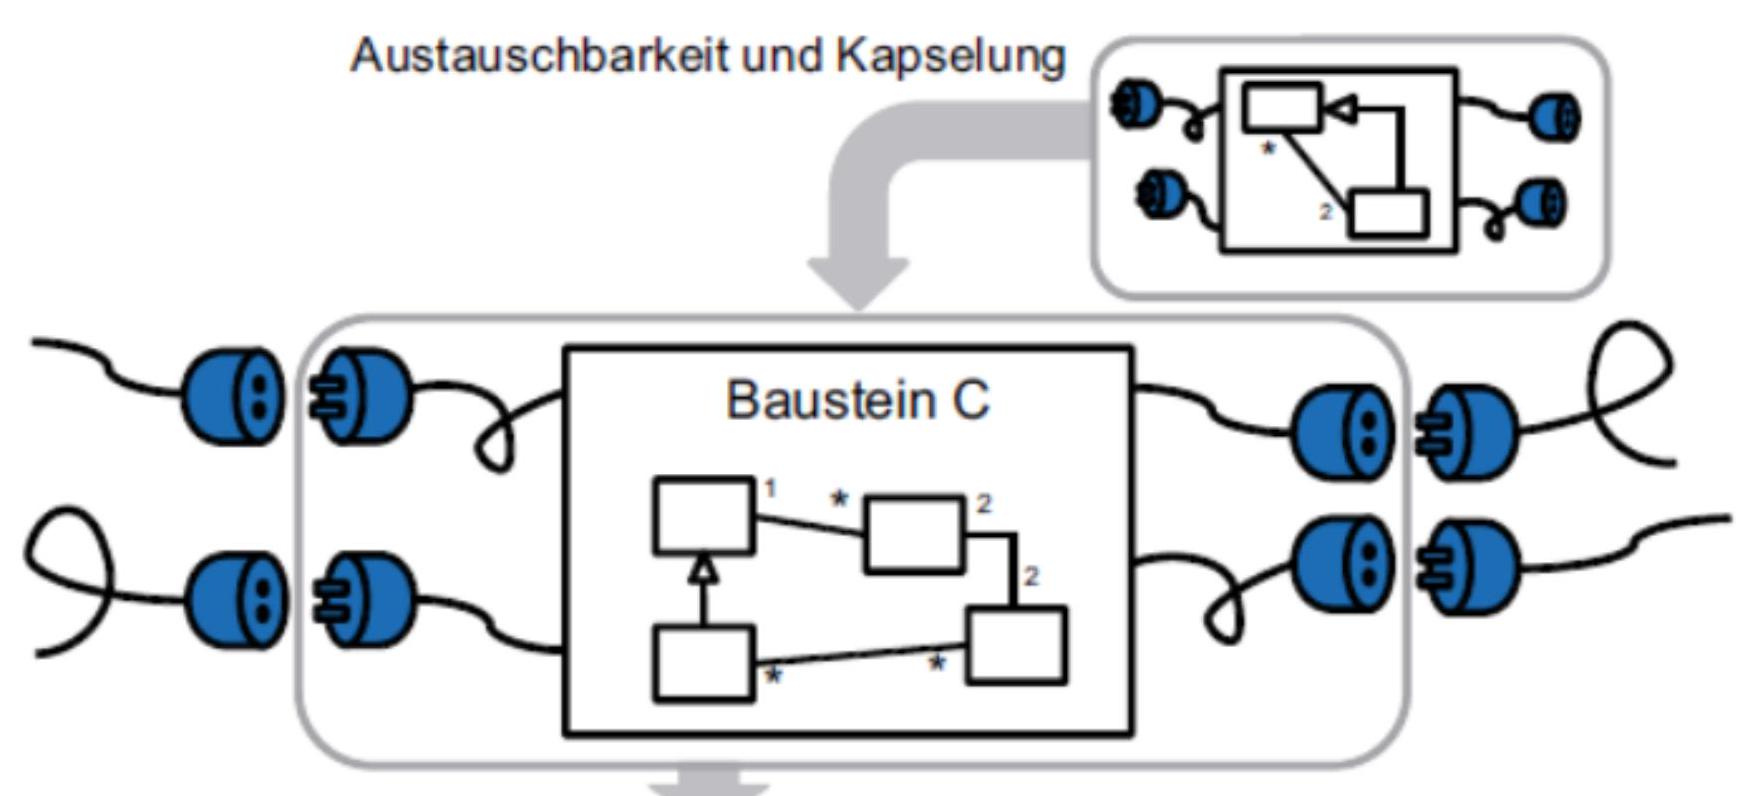
\includegraphics[max width=\textwidth, center]{2025_01_02_bc08e794b8341102ce21g-15}
\end{itemize}

\section*{Das Prinzip einer modularen Struktur}
\begin{itemize}
  \item Zwischen den Modulen
  \item Möglichst schwache Kopplung
  \item Kommunikation nur über Schnittstellen
  \item Innerhalb eines Moduls
  \item Alle Funktionalitäten und Daten, die benötigt werden
  \item von aussen nicht sichtbar
  \item meist starker Zusammenhang\\
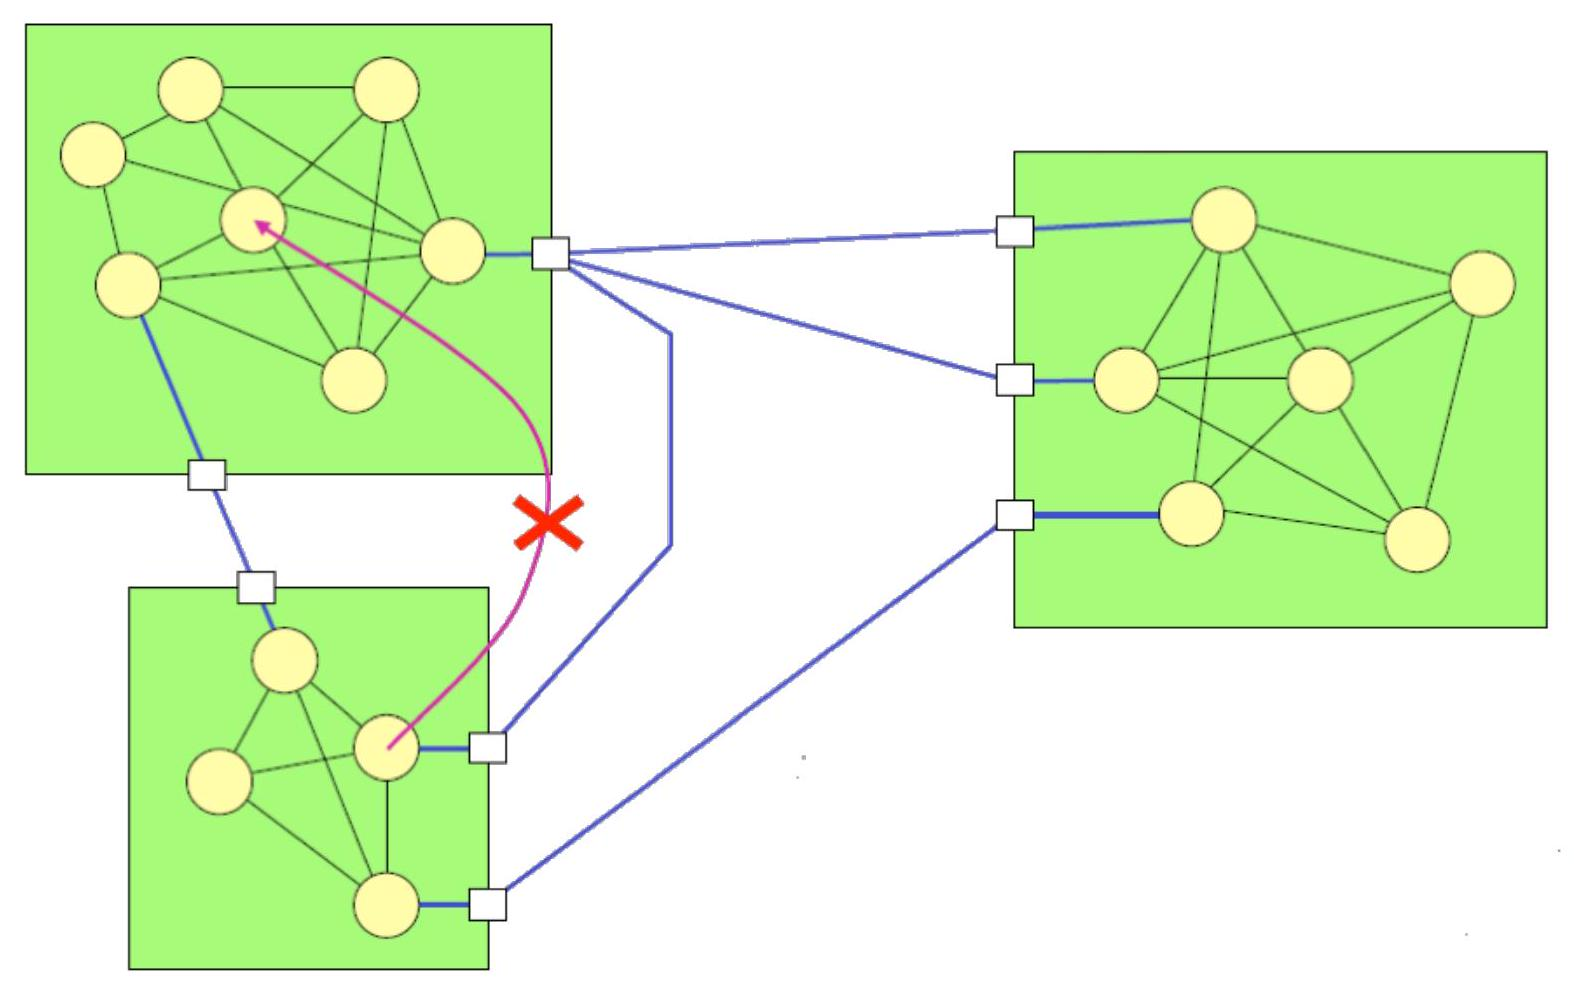
\includegraphics[max width=\textwidth, center]{2025_01_02_bc08e794b8341102ce21g-16}
\end{itemize}

\section*{Messung der Güte einer Modularisierung}
\begin{itemize}
  \item Zwei charakteristische Masse: Kohäsion und Kopplung (-> GRASP LE 06)
  \item Kohäsion
  \item Ein Mass für die Stärke des inneren Zusammenhangs
  \item Je höher die Kohäsion innerhalb eines Moduls, desto besser die Modularisierung
  \item schlecht: zufällig, zeitlich
  \item gut: funktional, objektbezogen
  \item Kopplung - Ein Mass für die Abhängigkeit zwischen zwei Modulen.
  \item Je geringer die wechselseitige Kopplung zwischen den Modulen, desto besser die Modularisierung
  \item schlecht: Globale Kopplung (Globale Daten)
  \item akzeptabel: Datenbereichskopplung (Referenzen auf gemeinsame Daten)
  \item gut: Datenkopplung (alle Daten werden beim Aufruf der Schnittstelle übergeben)
\end{itemize}

\begin{enumerate}
  \item Was ist eine Softwarearchitektur
  \item Architektur aus den Anforderungen ableiten
  \item Modulkonzept
  \item Architekturen beschreiben
  \item UML-Paketdiagramme
  \item Ausgewählte Architekturpatterns und Beispielarchitekturen
  \item Aufgaben eines Software-Architekten
  \item Wrap-up und Ausblick
\end{enumerate}

\section*{Architekturen beschreiben}
\begin{itemize}
  \item Architektur umfasst verschiedene Aspekte, die je nach Sichtweise wichtig sind
  \item Architekturbeschreibungen sind deshalb in verschiedene Sichten (Views) aufgeteilt
  \item Sichten sind Projektionen der Softwarearchitektur
  \item Beschreiben die Architektur aus einer bestimmten Sicht
  \item Die anderen Aspekte werden ausgeblendet
  \item Je nach Aufgabe benötigen Stakeholder (Interessenvertreter) eine unterschiedliche Sicht auf die Architektur
  \item Philippe Kruchten, 1995: 4 + 1 View Model
  \item Logical View:
  \item Welche Funktionalität bietet das System gegen aussen an?
  \item Wichtige Aspekte: Schichten, Subsysteme, Pakete, Frameworks, Klassen, Interfaces
  \item UML: Systemsequenzdiagramme, Interaktionsdiagramme, Klassendiagramm, Zustandsdiagramme
\end{itemize}

\section*{- Process View:}
\begin{itemize}
  \item Welche Prozesse laufen wo und wie ab im System?
  \item Wichtige Aspekte: Prozesse, Threads, Wie werden Anforderungen wie Performance und Stabilität erreicht?
  \item UML: Klassendiagramme, Interaktionsdiagramme, Aktivitätsdiagramme.\\
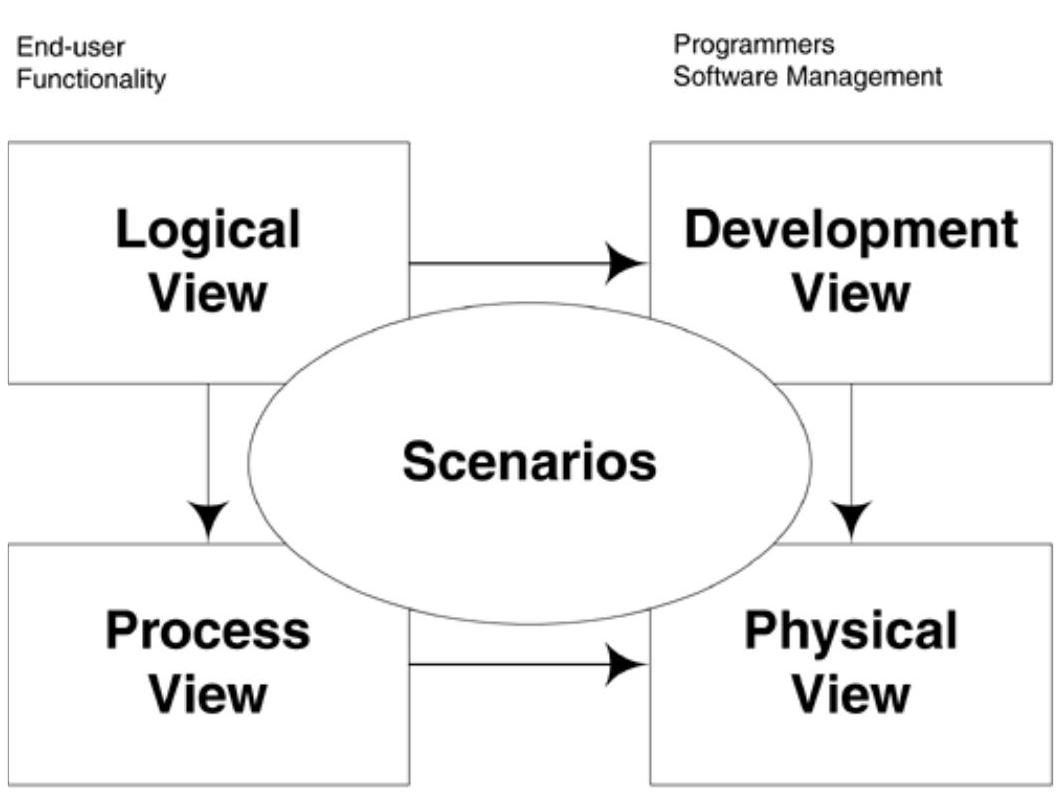
\includegraphics[max width=\textwidth, center]{2025_01_02_bc08e794b8341102ce21g-20}
\end{itemize}

Integrators\\
Performance\\
Scalability\\
Systems engineers\\
Topology\\
Communications

\footnotetext{Philippe Kruchten, 1995:\\
\href{http://www.cs.ubc.ca/~gregor/teaching/papers/4+1vie}{http://www.cs.ubc.ca/\~{}gregor/teaching/papers/4+1vie} w-architecture.pdf
}\begin{itemize}
  \item Development View (Implementation View):
  \item Wie wurde die logische Struktur (Layer, Schichten, Komponenten) umgesetzt?
  \item Wichtige Aspekte: Source Code, Executables, Artefakte
  \item UML: Paketdiagramme, Komponentendiagramme
  \item Physical View (Deployment View):
  \item Auf welcher Infrastruktur wird ein System ausgeliefert/betrieben?
  \item Wichtige Aspekte: Prozessknoten, Netzwerke, Protokolle
  \item UML: Deployment Diagram
\end{itemize}

End-user\\
Functionality

Programmers\\
Software Management\\
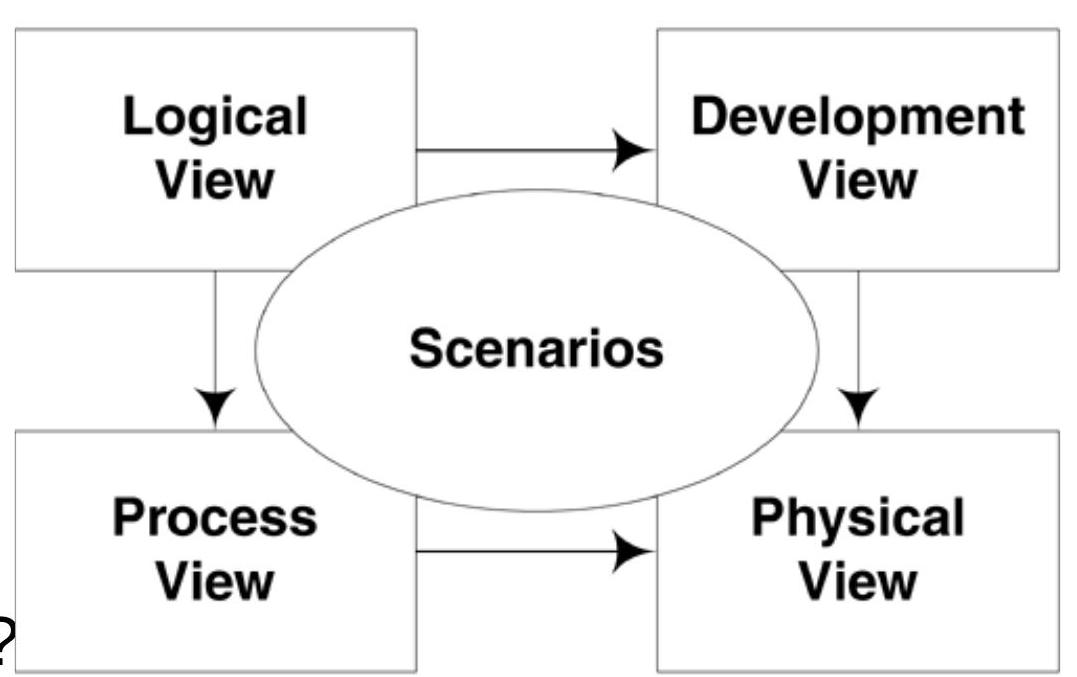
\includegraphics[max width=\textwidth, center]{2025_01_02_bc08e794b8341102ce21g-21}

\section*{Das N+1 View Model}
\begin{itemize}
  \item «+1» View: Scenarios (Use Cases)
  \item Welches sind die wichtigsten Use-Cases und ihre nichtfunktionalen Anforderungen? Wie wurden sie umgesetzt?
  \item Wichtige Aspekte: Architektonisch wichtige UCs, deren nichtfunktionale Anforderungen und deren Implementation
  \item UML: UC-Diagramm, Systemsequenzdiagramme, UCRealisierungen
  \item Weitere mögliche Views
\end{itemize}

Integrators\\
Performance\\
Scalability

End-user\\
Functionality

Programmers\\
Software Management\\
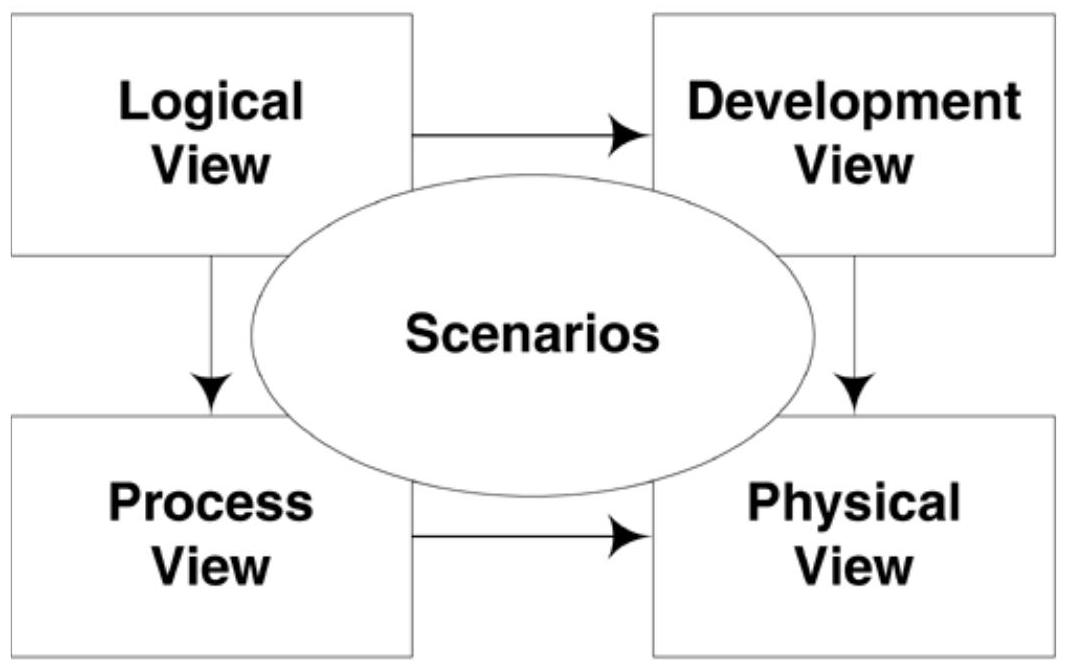
\includegraphics[max width=\textwidth, center]{2025_01_02_bc08e794b8341102ce21g-22}

Systems engineers\\
Topology\\
Communications

\begin{itemize}
  \item Daten-Sicht
  \item Sicherheit
\end{itemize}

Philippe Kruchten, 1995:\\
\href{http://www.cs.ubc.ca/~gregor/teaching/papers/4+1vie}{http://www.cs.ubc.ca/\~{}gregor/teaching/papers/4+1vie} w-architecture.pdf

\begin{enumerate}
  \item Was ist eine Software Architektur
  \item Grundlagen für die Architektur aus den Anforderungen ableiten
  \item Modulkonzept
  \item Architekturen beschreiben
  \item UML-Paketdiagramme und Verteilungsdiagramm
  \item Ausgewählte Architekturpatterns und Beispielarchitekturen
  \item Wrap-up und Ausblick
\end{enumerate}

\section*{UML-Paketdiagramme}
\begin{itemize}
  \item UML-Paketdiagramme werden häufig zur Dokumentation der Architektur verwendet
  \item Mittel, um Teilsysteme zu definieren
  \item Mittel zur Gruppierung von Elementen
  \item Paket enthält Klassen und andere Pakete
  \item Ähnlich, aber allgemeiner als Java Packages
  \item Abhängigkeiten zwischen Paketen\\
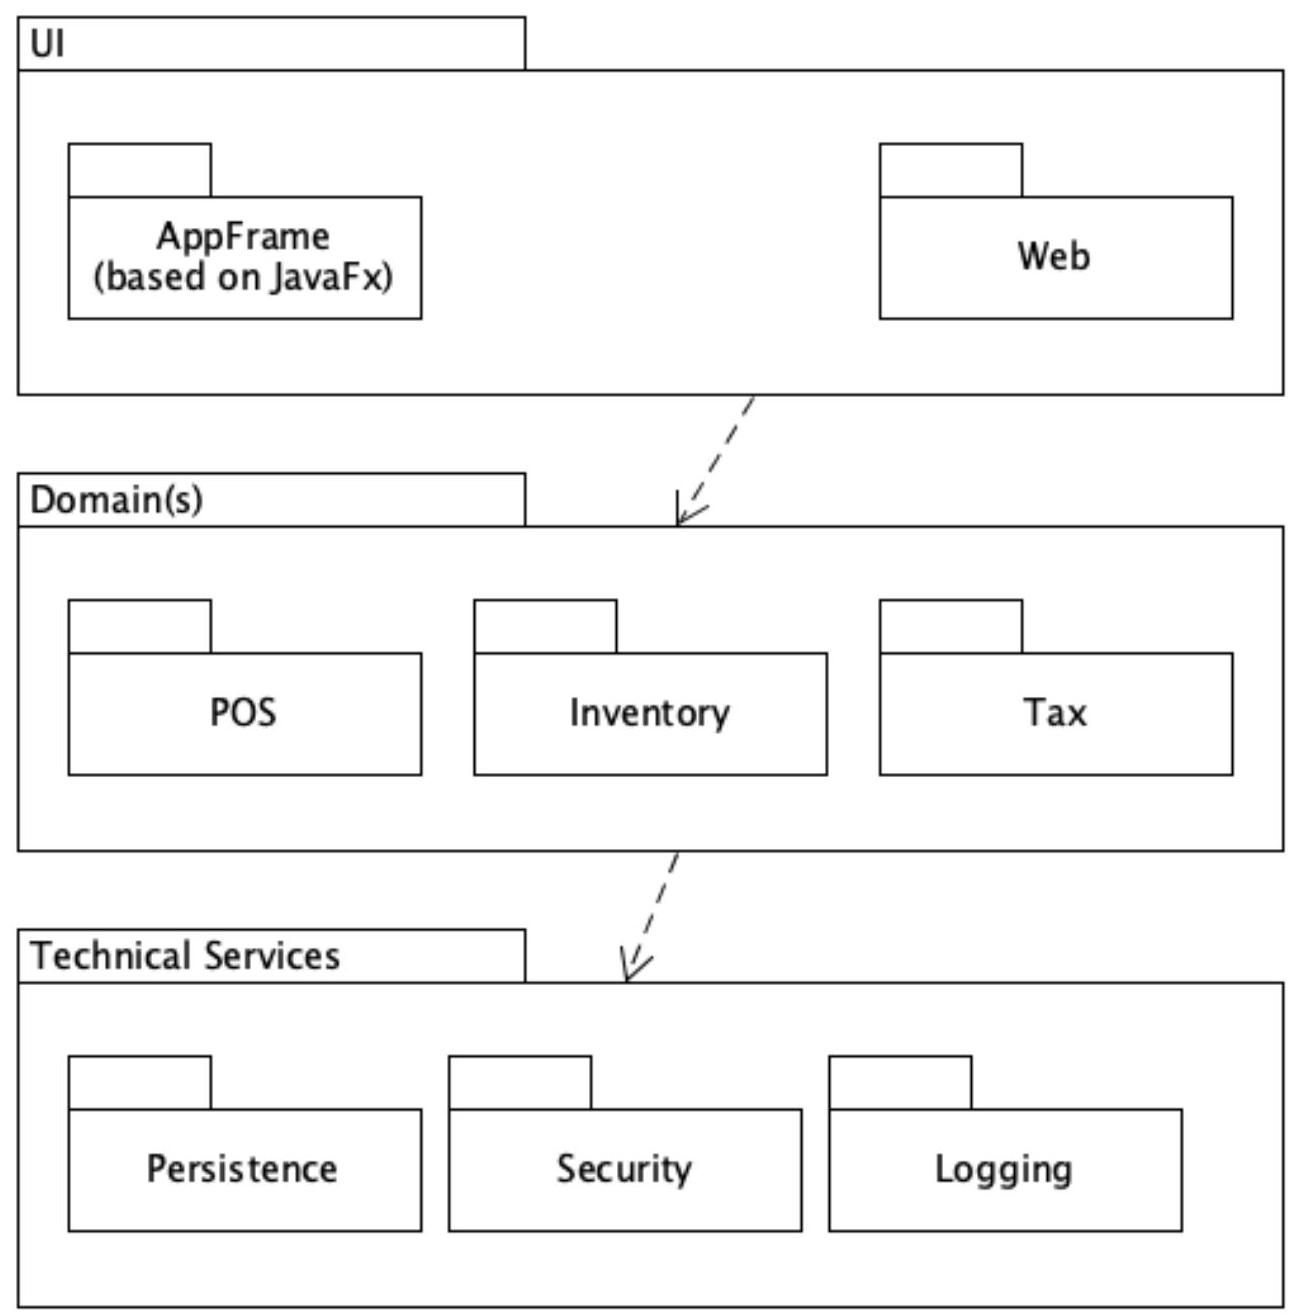
\includegraphics[max width=\textwidth, center]{2025_01_02_bc08e794b8341102ce21g-24}
\end{itemize}

\section*{UML-Paketdiagramme: Tier, Layer (Schicht) und Partition}
\begin{itemize}
  \item Layer: logische Struktur
  \item Unabhängig betreffend Ausführung
  \item Physical Tier
  \item auf welchem Rechnerknoten
  \item Partition
  \item Unterteilung in einzelne Themen\\
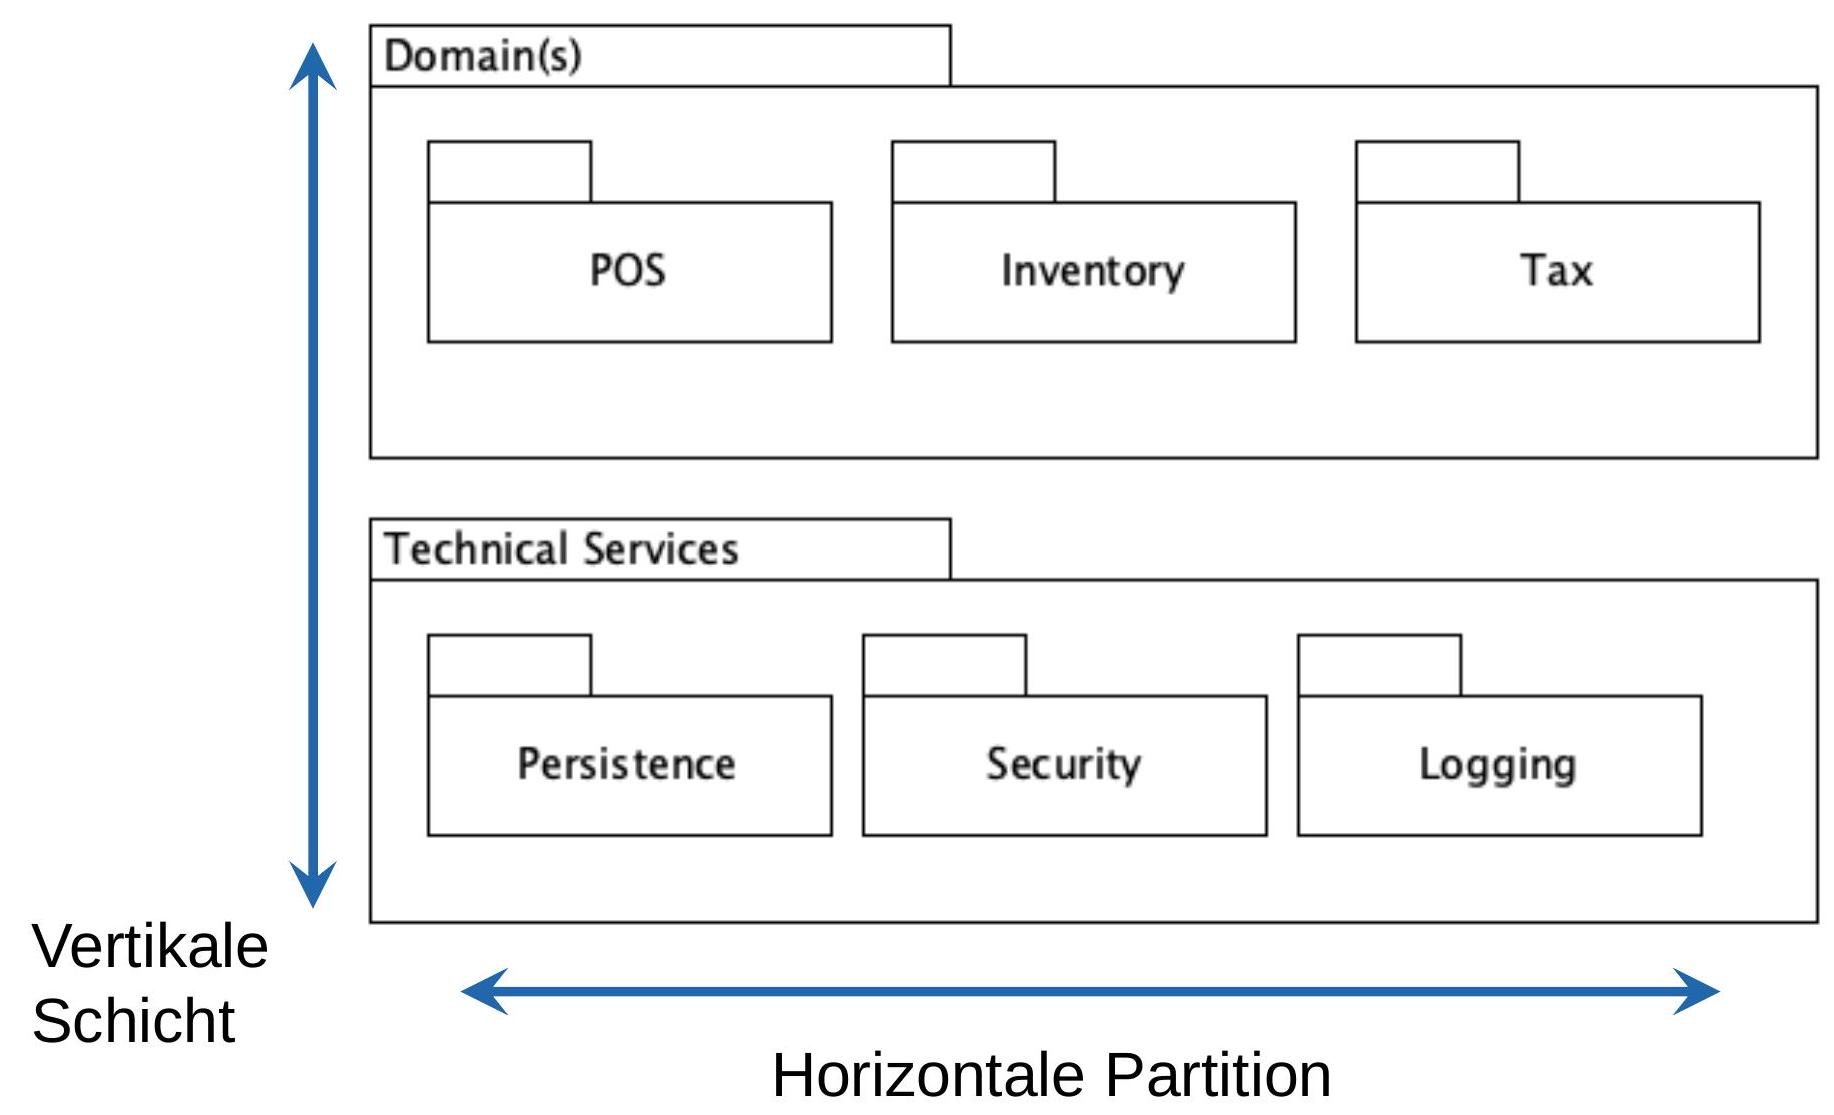
\includegraphics[max width=\textwidth, center]{2025_01_02_bc08e794b8341102ce21g-25}
\end{itemize}

\section*{Pakete umsetzen}
\begin{itemize}
  \item Java: Packages
  \item com.mycompany.nextgen.ui.swing
  \item com.mycompany.nextgen.domain.sales
  \item com.mycompany.service.persistence
  \item org.apache.log4j
  \item C\# : Namensräume und Assemblies
  \item Tipp für wiederverwendbare Pakete: Keine projektspezifischen Namen
\end{itemize}

\section*{Verteilungsdiagramm}
\begin{itemize}
  \item Das Verteilungsdiagramm
  \item dient der Darstellung der Verteilung von Komponenten auf Rechenknoten mit Abhängigkeiten, Schnittstellen und Verbindungen
  \item gehört zu den Diagrammen der statischen Modellierung\\
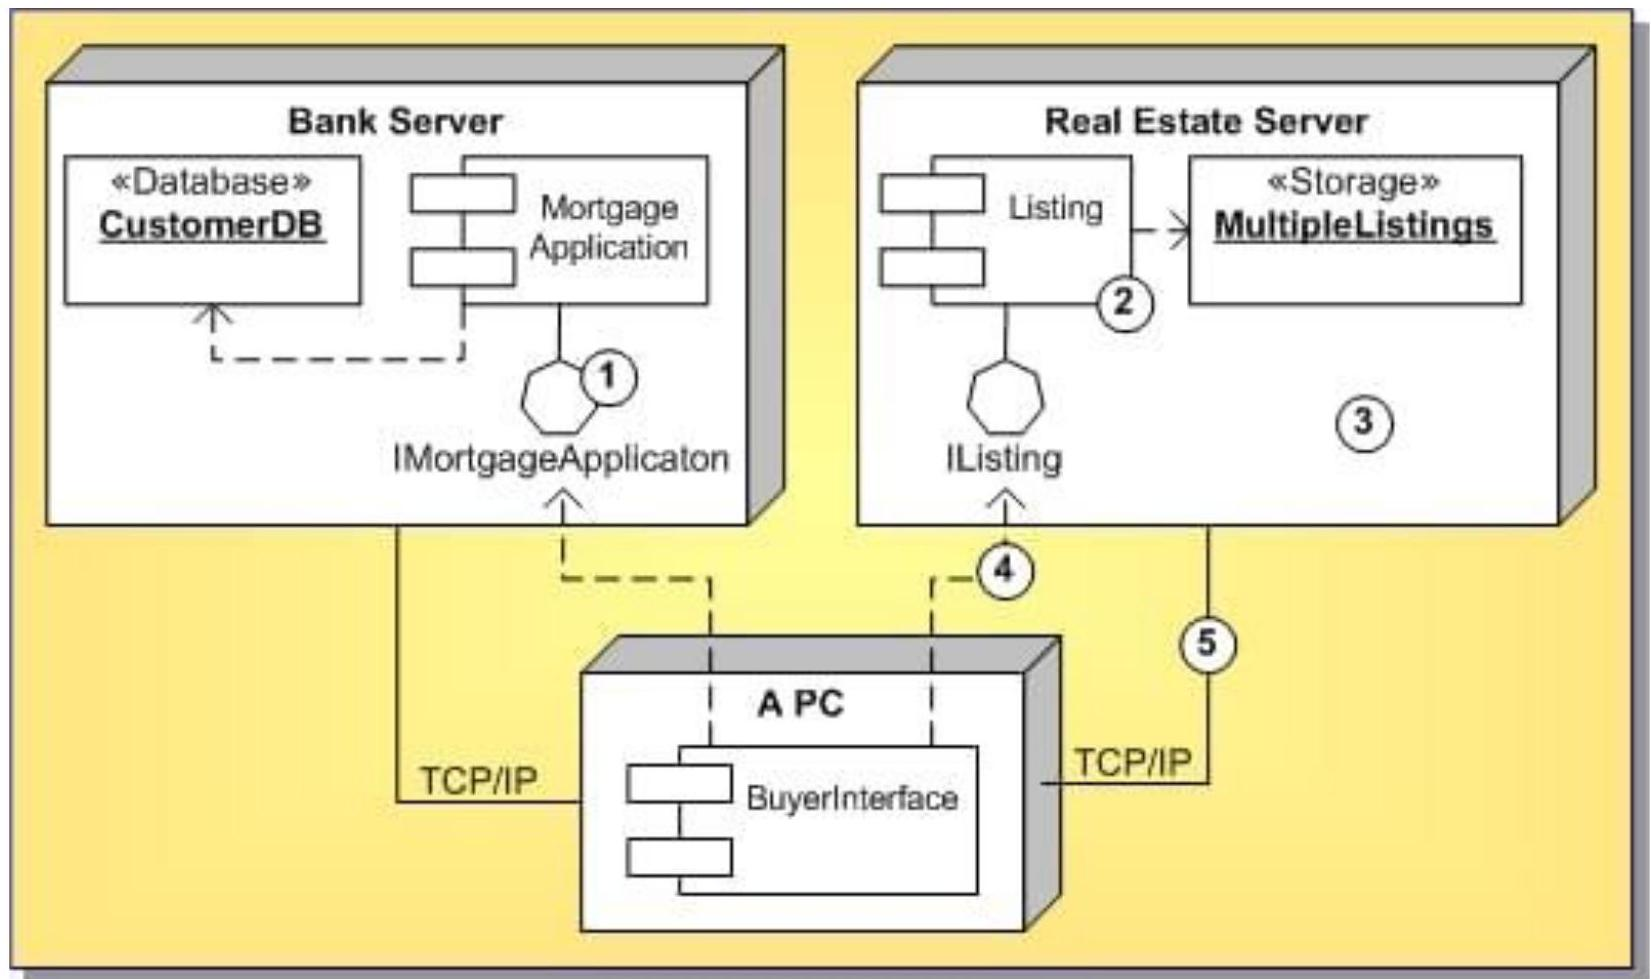
\includegraphics[max width=\textwidth, center]{2025_01_02_bc08e794b8341102ce21g-27}\\
(1) Interface (2) Component (3) Node (4) Dependency (5) Connection
\end{itemize}

\begin{enumerate}
  \item Was ist eine Software Architektur
  \item Grundlagen für die Architektur aus den Anforderungen ableiten
  \item Modulkonzept
  \item Architekturen beschreiben
  \item UML-Paketdiagramme
  \item Ausgewählte Architekturpatterns und Beispielarchitekturen
  \item Wrap-up und Ausblick
\end{enumerate}

\section*{Ausgewählte Architekturpatterns}
\begin{center}
\begin{tabular}{|ll|}
\hline
Pattern & Beschreibung \\
\hline
Layered Pattern & Strukturierung eines Programms in Schichten \\
\hline
Client-Server Pattern & Ein Server stellt Services für mehrere Clients zur Verfügung \\
\hline
Master-Slave Pattern & Ein Master verteilt die Arbeit auf mehrere Slaves \\
\hline
Pipe-Filter Pattern & Verarbeitung eines Datenstroms (filtern, zuordnen, speichern) \\
\hline
Broker Pattern & Meldungsvermittler zwischen verschiedenen Endpunkten \\
\hline
Event-Bus Pattern & \begin{tabular}{l}
Datenquellen publizieren Meldungen an einen Kanal auf dem Event-Bus. \\
Datensenken abonnieren einen bestimmten Kanal \\
\end{tabular} \\
\hline
MVC Pattern & \begin{tabular}{l}
Eine interaktive Anwendung wird in 3 Komponenten aufgeteilt: \\
Model, View - Informationsanzeige, Controller - Verarbeitung der \\
Benutzereingabe \\
\end{tabular} \\
\hline
\end{tabular}
\end{center}

\begin{itemize}
  \item Unter dem von Uncle Bob (Robert C. Martin) geprägten Begriff versteht man
  \item Unabhängigkeit von einem bestimmten Framework
  \item Business Rules können unabhängig von UI, DB, Web Server getestet werden
  \item Unabhängig von einem bestimmten UI\\
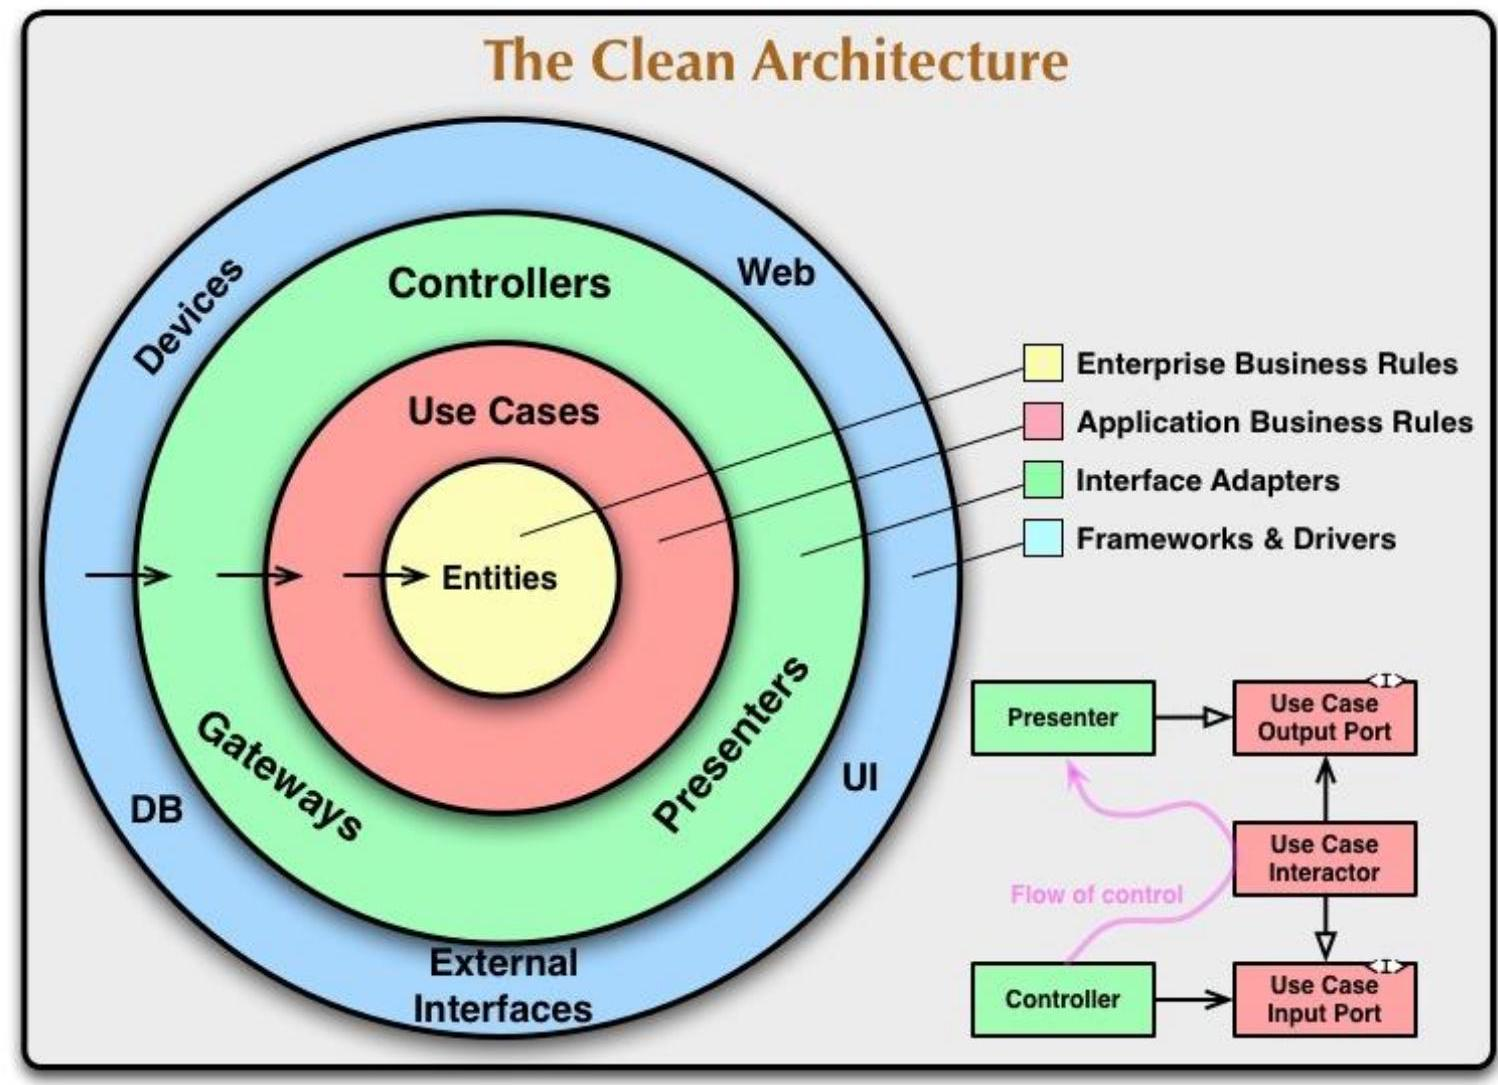
\includegraphics[max width=\textwidth, center]{2025_01_02_bc08e794b8341102ce21g-30}
  \item Unabhängig von einer bestimmten DB
  \item Entities
  \item Kapseln die Business Rules gültig für das gesamte Unternehmen
  \item Use Cases
  \item Beinhalten die Business Rules einer Anwendung, orchestriert die Verwendung der Entities
  \item Interface Adapters
  \item Adapter für die Konvertierung von\\
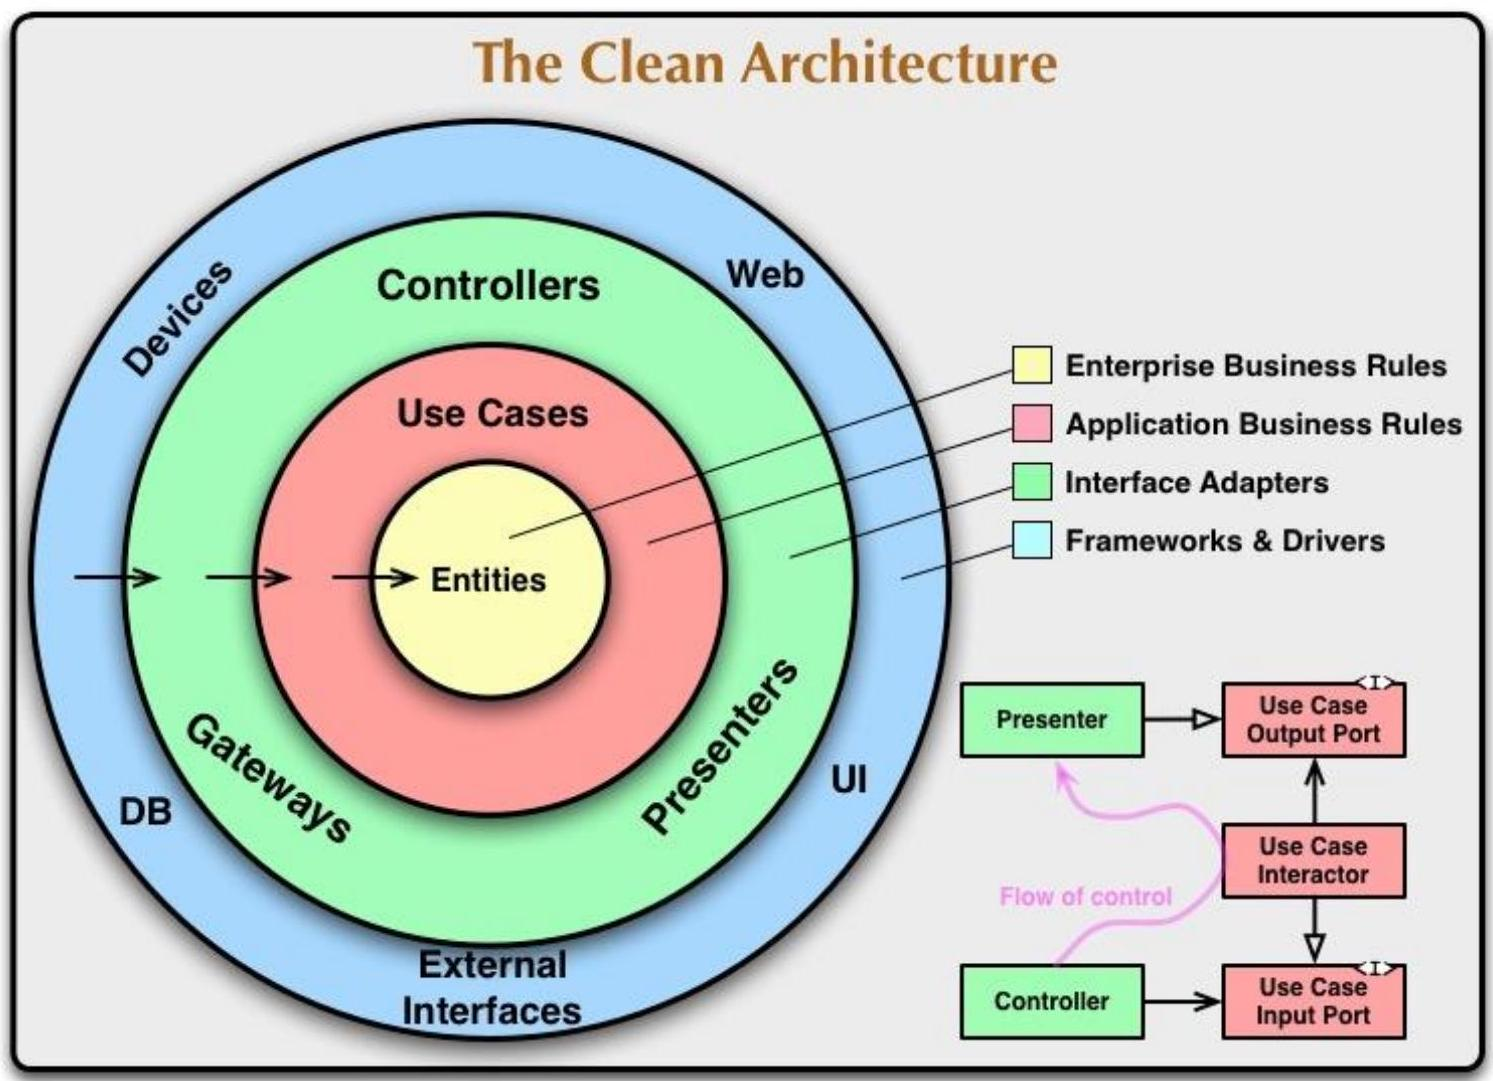
\includegraphics[max width=\textwidth]{2025_01_02_bc08e794b8341102ce21g-31} Daten aus Datenbank oder Web
\end{itemize}

\section*{- Frameworks and Drivers}
\section*{Clean Architecture Bemerkungen}
\begin{itemize}
  \item Die Domänenlogik hat keine Abhängigkeiten zu externem Code
  \item Frameworks, technische Services, Bibliotheken
  \item Externe Dienste, UI, Testcode
  \item Beurteilung
  \item Vieles wird heute als «Best Practice» angeschaut und ist auch so im Schichtenkonzept umgesetzt.
  \item Es gibt aber kaum ein Projekt, das «Clean Architecture» vollständig umsetzt. Gewisser externer Code wird immer integriert.
  \item Platform Code (z.B. Java Bibliotheken) und Libraries mit engem Funktionsumfang ist eher unproblematisch.
  \item Frameworks sollten zurückhaltend eingesetzt und sorgfältig ausgewählt werden.
\end{itemize}

\section*{Clean Architecture im Schichtenkonzept}
School of\\
Engineering\\
InIT Institut für angewandte Informationstechnologie\\
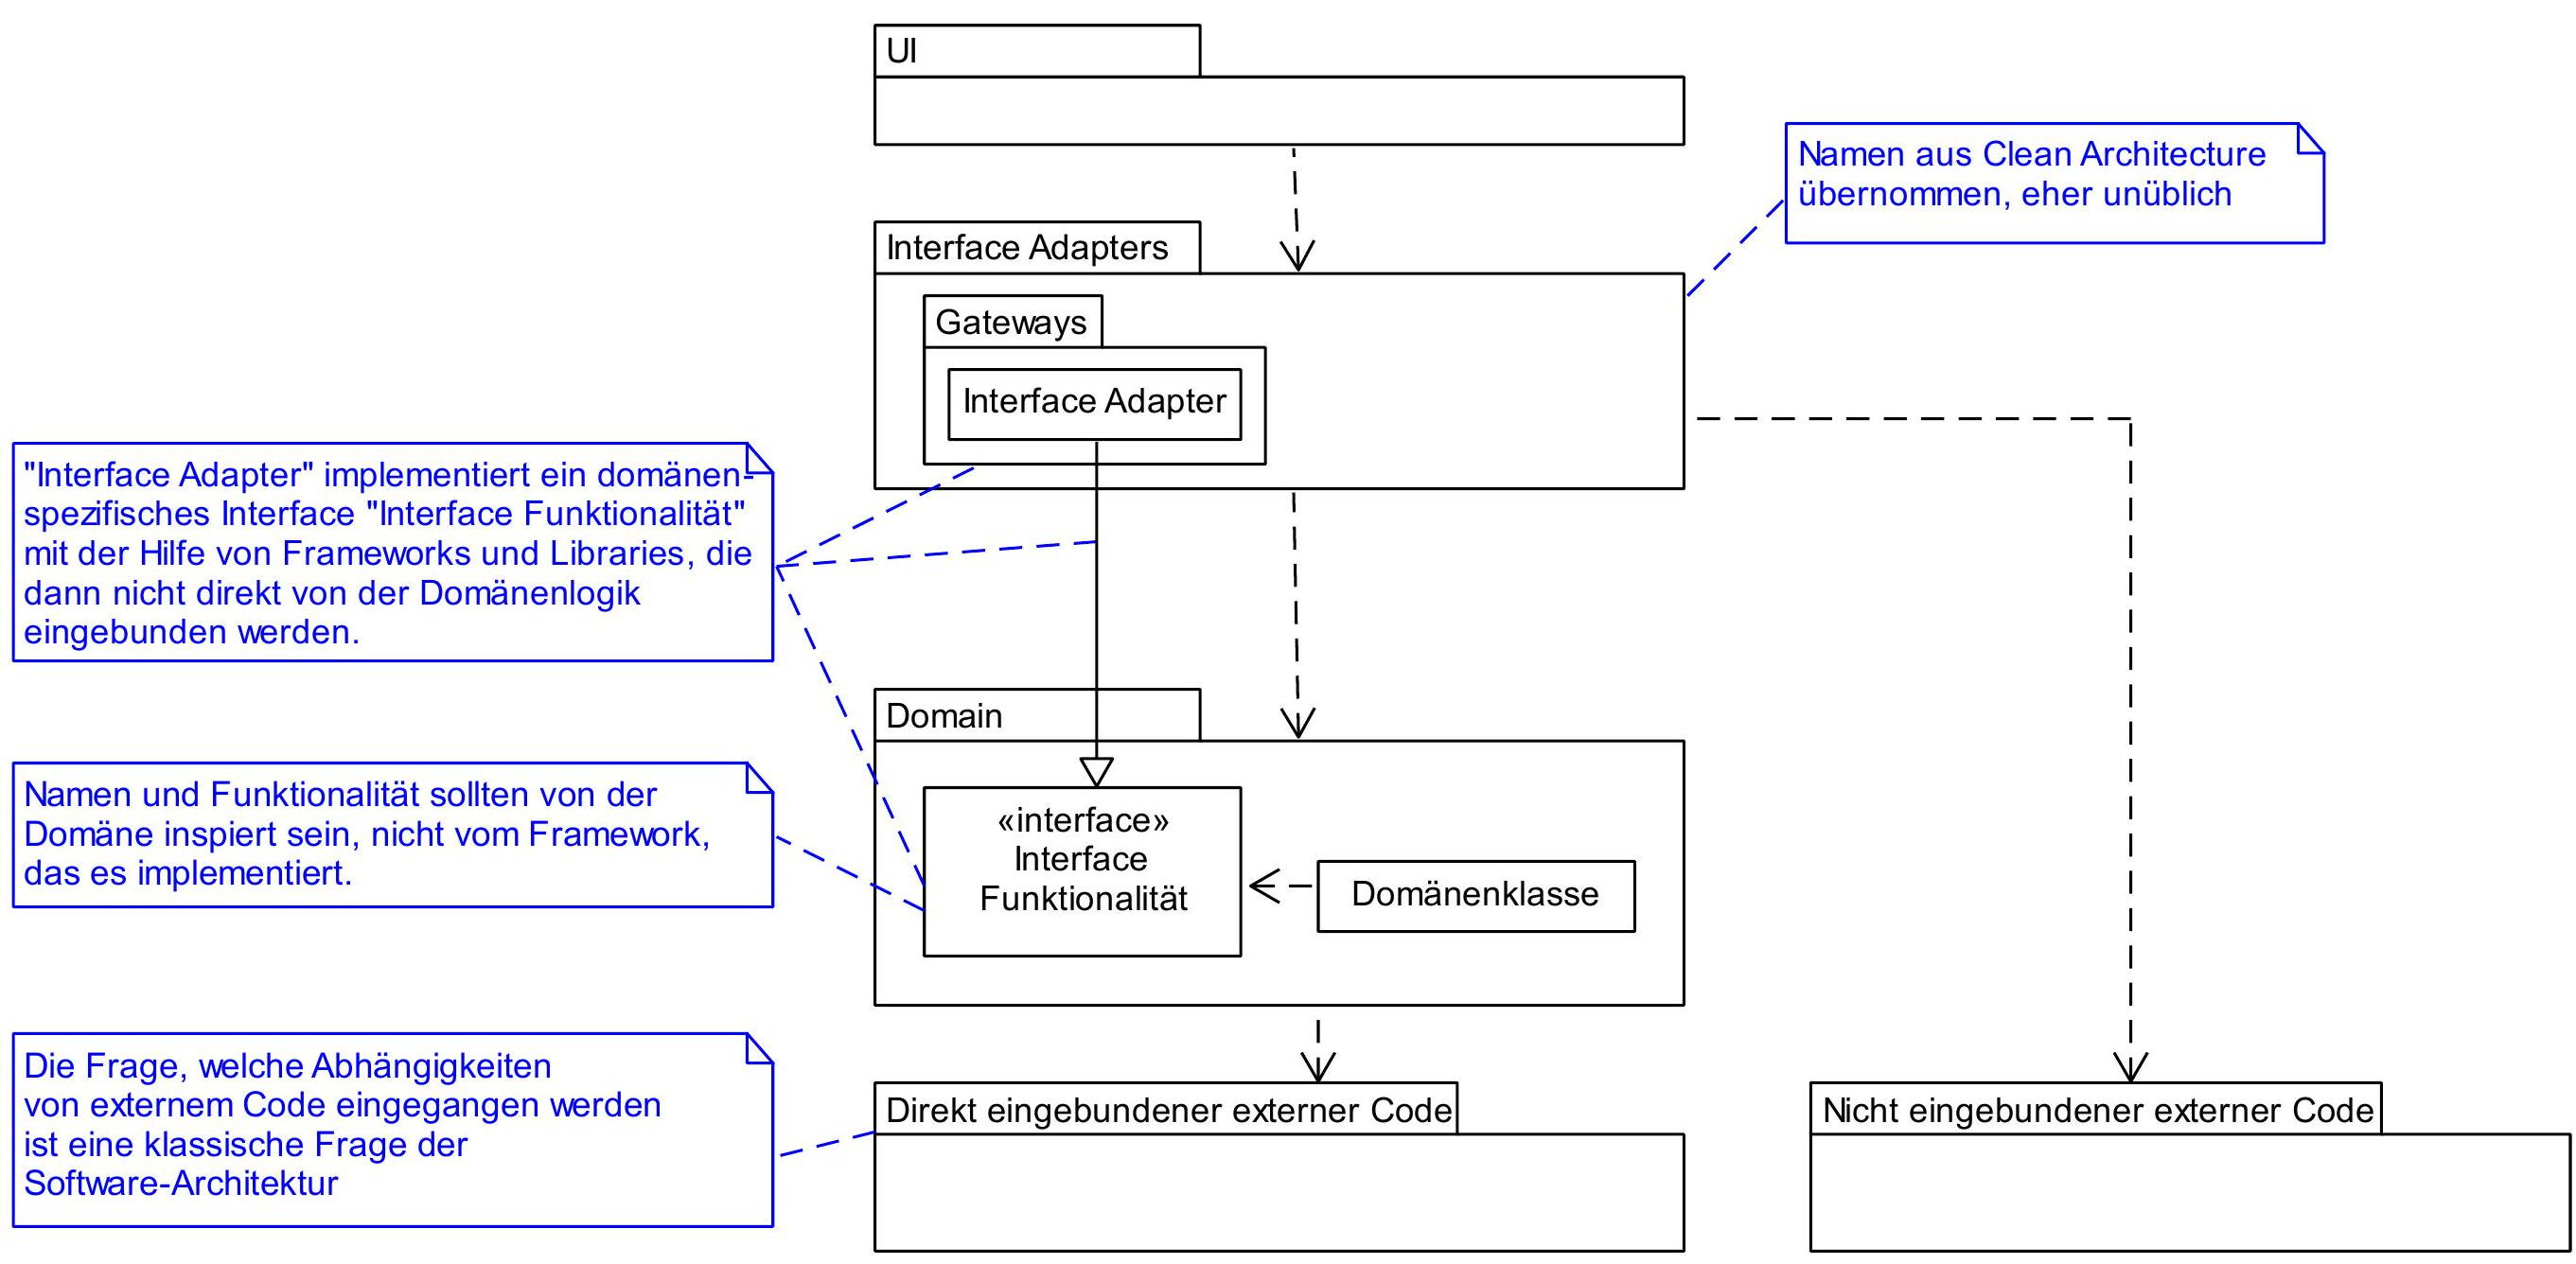
\includegraphics[max width=\textwidth, center]{2025_01_02_bc08e794b8341102ce21g-33}

\section*{Kritische Bemerkungen zu Frameworks}
\begin{itemize}
  \item Frameworks tendieren dazu, im Laufe der Zeit immer mehr Funktionalität zu «sammeln».
  \item Was auf den ersten Blick positiv scheint, kann im zweiten Blick zu inkonsistentem Design und funktionalen Überschneidungen führen, die den Einsatz immer mehr erschweren.
  \item Der Einsatz eines Frameworks sollte gut überlegt werden.
  \item Einerseits erfordert dies gute Kenntnisse des Frameworks, andererseits ist nach der «Verheiratung» der Anwendung mit dem Framework eine «Scheidung» nur noch schwierig und mit hohem Aufwand möglich.
  \item Allenfalls sollte das Framework nur über eigene Schnittstellen verwendet werden (keine direkte Abhängigkeit), was aber unter Umständen die Nützlichkeit des Einsatzes in Frage stellt.
\end{itemize}

\begin{enumerate}
  \item Was ist eine Software Architektur
  \item Grundlagen für die Architektur aus den Anforderungen ableiten
  \item Modulkonzept
  \item Architekturen beschreiben
  \item UML-Paketdiagramme
  \item Ausgewählte Architekturpatterns und Beispielarchitekturen
  \item Wrap-up und Ausblick
\end{enumerate}

\begin{itemize}
  \item Die Softwarearchitektur definiert die grundlegenden Prinzipien und Regeln für die Organisation eines Systems sowie dessen Strukturierung in Bausteinen und Schnittstellen und deren Beziehungen zueinander wie auch zur Umgebung.
  \item Zentrale Aufgabe der Architekturanalyse ist es, die funktionalen und insbesondere nichtfunktionalen Anforderungen als Grundlage für den Entwurf der Softwarearchitektur zu untersuchen.
  \item Eine Softwarearchitektur wird aus verschiedenen Sichten beschrieben.
  \item Eine logische Software-Architektur wird mit einem UML-Paketdiagramm dargestellt.
  \item Es gibt verschiedene Architekturpatterns, die eine Standardarchitektur für eine bestimmte Problemstellungen bieten (Layered Pattern, Client-Server, MasterSlave etc.).
  \item In der nächsten Lerneinheit werden wir folgende Fragen behandeln:
  \item Wie modelliere ich mein Design mit der UML, um es diskutieren und evaluieren zu können?
  \item Wie realisiere ich einen Use Case mit Klassen, die klare Verantwortlichkeiten haben, wartbar und einfach erweiterbar sind?
\end{itemize}

\section*{Quellenverzeichnis}
[1] Larman, C.: UML 2 und Patterns angewendet, mitp Professional, 2005\\[0pt]
[2] Seidel, M. et al.: UML @ Classroom: Eine Einführung in die objektorientierte Modellierung, dpunkt.verlag, 2012\\[0pt]
[3] Martin, R. C.: Clean Architecture: A Craftsman's Guide to Software Structure and Design, mitp Professional, 2018


\end{document}